\section{MaxContext}
\label{sec:methodology}

% Style note (v2, 2026-05-07): tightened to ~400 words + Algorithm 1 to fit the 0.7-page budget per plan v4. Adopts the Outstanding-paper convention of question-style or claim-style section titles where it improves clarity; here the section is named after the method itself, matching the method-named title.

\paragraph{Reranking Setup.}
Given a query $q$ and a first-stage BM25 run~\citep{robertson2009probabilistic}, let $P=(d_1,\ldots,d_N)$ denote the top-$N$ candidate pool in BM25 order. The task is to produce a full reranking $R=(r_1,\ldots,r_N)$ from which nDCG@10~\citep{jarvelin2002cumulated} is computed on the prefix. We study the matched operating point $k=N$ for all methods, and for MaxContext an initial prompt window $W=N$: the entire reranking pool is visible in the first LLM call. Passages are rendered with passage length $\ell{=}512$. A runtime tokenization preflight then verifies that the rendered prompt fits the model context window; prompts are not truncated.

\paragraph{Compared Methods.}
Our method axis contains seven rerankers. Four are standard setwise baselines following the local-window formulation of \citet{zhuang2024setwise}: TopDown setwise with bubblesort, TopDown setwise with heapsort, BottomUp setwise with bubblesort, and BottomUp setwise with heapsort, all using the public \texttt{llm-rankers} implementation~\citep{ielab_llmrankers}. The remaining three are MaxContext variants: best-only \textsc{MaxContext-TopDown}, worst-only \textsc{MaxContext-BottomUp}, and joint best--worst \textsc{MaxContext-DualEnd}. Standard DualEnd sorting baselines are not part of this method matrix.

\paragraph{MaxContext Skeleton.}
MaxContext maintains a live pool $L$, initialized to the BM25 top-$N$ list $P$. Every LLM call sees the query and every document in the current $L$. Documents are addressed by local numeric labels $1,\ldots,|L|$, which replace the fixed-letter interface of windowed setwise and allow the whole live pool to be referenced when $|L|$ exceeds the letter range. Outputs are strictly parsed as integer labels: a single-extreme call accepts exactly one integer in $[1,|L|]$, a dual-end call accepts exactly two distinct integers in $[1,|L|]$. Out-of-range, duplicate, or missing labels and refusal-like outputs are recorded as parse failures and invalidate the run --- we do not repair such outputs with fallback heuristics. Every successful MaxContext run thus returns a true permutation of the original BM25 pool.

\paragraph{Three Variants.}
\textsc{MaxContext-TopDown} asks for the best document, places it at the next free head of $R$, and removes it from $L$. \textsc{MaxContext-BottomUp} asks for the worst, places it at the next free tail, and removes it. Both single-extreme variants stop when two documents remain and order the residual pair deterministically by BM25 (higher above lower). \textsc{MaxContext-DualEnd} asks for both extremes in the same call, placing one at the head and one at the tail and removing both per call; Algorithm~\ref{alg:dualend} formalizes the loop and Figure~\ref{fig:dualend} traces a worked $N{=}10$ run.

\begin{figure}[t]
\centering
\scriptsize
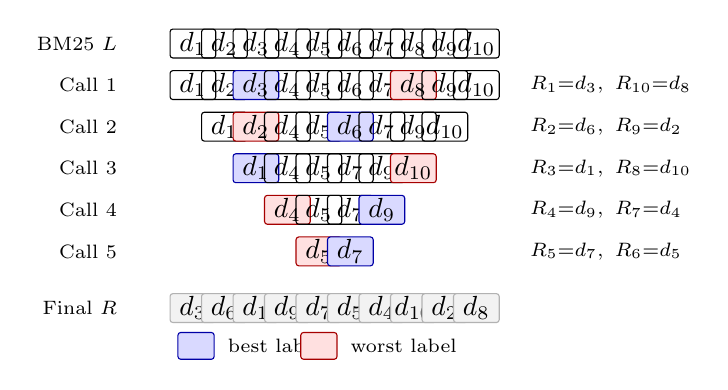
\begin{tikzpicture}[
  x=0.40cm,
  y=0.48cm,
  doc/.style={draw, rounded corners=1pt, minimum width=0.58cm, minimum height=0.34cm, inner sep=1pt},
  best/.style={doc, fill=blue!15, draw=blue!65!black},
  worst/.style={doc, fill=red!12, draw=red!65!black},
  placed/.style={doc, fill=gray!10, draw=gray!60},
  label/.style={anchor=east, font=\scriptsize},
  note/.style={anchor=west, font=\scriptsize}
]

\node[label] at (-1.1,0) {BM25 $L$};
\foreach \d [count=\i from 1] in {1,2,3,4,5,6,7,8,9,10} {
  \node[doc] at (\i,0) {$d_{\d}$};
}

\node[label] at (-1.1,-1.1) {Call 1};
\foreach \d [count=\i from 1] in {1,2,3,4,5,6,7,8,9,10} {
  \ifnum\d=3
    \node[best] at (\i,-1.1) {$d_{\d}$};
  \else
    \ifnum\d=8
      \node[worst] at (\i,-1.1) {$d_{\d}$};
    \else
      \node[doc] at (\i,-1.1) {$d_{\d}$};
    \fi
  \fi
}
\node[note] at (11.4,-1.1) {$R_1{=}d_3,\ R_{10}{=}d_8$};

\node[label] at (-1.1,-2.2) {Call 2};
\foreach \d [count=\i from 1] in {1,2,4,5,6,7,9,10} {
  \ifnum\d=6
    \node[best] at (\i+1,-2.2) {$d_{\d}$};
  \else
    \ifnum\d=2
      \node[worst] at (\i+1,-2.2) {$d_{\d}$};
    \else
      \node[doc] at (\i+1,-2.2) {$d_{\d}$};
    \fi
  \fi
}
\node[note] at (11.4,-2.2) {$R_2{=}d_6,\ R_9{=}d_2$};

\node[label] at (-1.1,-3.3) {Call 3};
\foreach \d [count=\i from 1] in {1,4,5,7,9,10} {
  \ifnum\d=1
    \node[best] at (\i+2,-3.3) {$d_{\d}$};
  \else
    \ifnum\d=10
      \node[worst] at (\i+2,-3.3) {$d_{\d}$};
    \else
      \node[doc] at (\i+2,-3.3) {$d_{\d}$};
    \fi
  \fi
}
\node[note] at (11.4,-3.3) {$R_3{=}d_1,\ R_8{=}d_{10}$};

\node[label] at (-1.1,-4.4) {Call 4};
\foreach \d [count=\i from 1] in {4,5,7,9} {
  \ifnum\d=9
    \node[best] at (\i+3,-4.4) {$d_{\d}$};
  \else
    \ifnum\d=4
      \node[worst] at (\i+3,-4.4) {$d_{\d}$};
    \else
      \node[doc] at (\i+3,-4.4) {$d_{\d}$};
    \fi
  \fi
}
\node[note] at (11.4,-4.4) {$R_4{=}d_9,\ R_7{=}d_4$};

\node[label] at (-1.1,-5.5) {Call 5};
\foreach \d [count=\i from 1] in {5,7} {
  \ifnum\d=7
    \node[best] at (\i+4,-5.5) {$d_{\d}$};
  \else
    \node[worst] at (\i+4,-5.5) {$d_{\d}$};
  \fi
}
\node[note] at (11.4,-5.5) {$R_5{=}d_7,\ R_6{=}d_5$};

\node[label] at (-1.1,-7.0) {Final $R$};
\foreach \d [count=\i from 1] in {3,6,1,9,7,5,4,10,2,8} {
  \node[placed] at (\i,-7.0) {$d_{\d}$};
}

\node[best, minimum width=0.46cm] at (1.1,-8.0) {};
\node[note] at (1.8,-8.0) {best label};
\node[worst, minimum width=0.46cm] at (5.0,-8.0) {};
\node[note] at (5.7,-8.0) {worst label};
\end{tikzpicture}
\caption{A ten-document run fills the ranking from both ends as the live pool shrinks.}
\label{fig:dualend}
\end{figure}


\begin{algorithm}[t]
\small
\caption{\textsc{MaxContext-DualEnd}}
\label{alg:dualend}
\begin{algorithmic}[1]
\State \textbf{Input:} query $q$, ordered BM25 top-$N$ pool $P=(d_1,\ldots,d_N)$
\State \textbf{Output:} full reranking $R$ of length $N$
\State $L \gets P$;\quad $R \gets$ empty array of length $N$
\State $\texttt{top} \gets 1$; \ $\texttt{bot} \gets N$
\While{$|L| \ge 2$}
  \State $y \gets \textsc{LLM}_{\mathrm{dual}}(q,L)$
  \State parse $y$ as $(i_{\mathrm{best}}, i_{\mathrm{worst}})$
  \Comment{distinct labels in $[1,|L|]$}
  \If{the parse is invalid}
    \State \textbf{abort}
  \EndIf
  \State $R[\texttt{top}] \gets L[i_{\mathrm{best}}]$;\ \ $R[\texttt{bot}] \gets L[i_{\mathrm{worst}}]$
  \State $\texttt{top} \gets \texttt{top}+1$;\ \ $\texttt{bot} \gets \texttt{bot}-1$
  \State delete $L[\max(i_{\mathrm{best}}, i_{\mathrm{worst}})]$
  \State delete $L[\min(i_{\mathrm{best}}, i_{\mathrm{worst}})]$
\EndWhile
\If{$|L| = 1$} \State $R[\texttt{top}] \gets L[1]$ \EndIf
\State \textbf{return} $R$
\end{algorithmic}
\end{algorithm}

\paragraph{LLM-Call Counts.}
At the matched operating point $W{=}k{=}N$, \textsc{DualEnd} uses $C_{\mathrm{DualEnd}}(N) = \lfloor N/2 \rfloor$ LLM calls, while either single-extreme variant uses $C_{\mathrm{TopDown}}(N) = C_{\mathrm{BottomUp}}(N) = N{-}2$ LLM calls plus one deterministic two-document BM25 endgame. At $N{=}100$, this is 50 vs.\ 98 calls; the ratio approaches $1/2$ from above as $N$ grows. Table~\ref{tab:call-accounting} reports the gap at representative $N$. The comparison is exact and within the MaxContext family; it is \emph{not} a claim that DualEnd halves tokens, FLOPs, or wall-clock --- those axes depend on prompt length, batching, and model throughput, which differ across variants.

\begin{table*}[t]
\centering
\small
\caption{MaxContext variants differ deterministically in serial LLM calls and residual BM25 handling. Top: per-variant accounting at pool size $N$. Bottom: concrete call counts at representative $N$.}
\label{tab:call-accounting}
\begin{tabular}{lcccc}
\toprule
\textbf{Variant} & \textbf{LLM calls} & \textbf{BM25 bypass} & \textbf{Serial decision steps} & \textbf{Pool shrinkage per call} \\
\midrule
\textsc{MaxContext-DualEnd} & $\lfloor N/2 \rfloor$ & $0$ & $\lfloor N/2 \rfloor$ & $2$ \\
\textsc{MaxContext-TopDown} & $N{-}2$ & $1$ & $N{-}1$ & $1$ \\
\textsc{MaxContext-BottomUp} & $N{-}2$ & $1$ & $N{-}1$ & $1$ \\
\bottomrule
\end{tabular}

\vspace{0.6em}

\begin{tabular}{lrrrr}
\toprule
\textbf{Pool size} & $N{=}10$ & $N{=}20$ & $N{=}50$ & $N{=}100$ \\
\midrule
\textsc{DualEnd} calls & 5 & 10 & 25 & 50 \\
Single-extreme calls & 8 & 18 & 48 & 98 \\
\bottomrule
\end{tabular}
\end{table*}


\paragraph{Hard Invariants.}
The EMNLP configuration fixes: $W=N=k$, $N\in\{10,20,30,40,50,100\}$, $\ell{=}512$, numeric one-based labels, strict context-fit preflight, no truncation, no parse-fallback repair, no permutation self-consistency, and generation-based scoring on causal LLMs from the Qwen3.5, Llama-3.1, and Ministral-3 families. Likelihood-scoring T5-style rerankers are excluded because the joint best--worst objective in DualEnd does not reduce to an independent single-label likelihood score without changing the method.
